\documentclass[12pt,fleqn,a4paper,oneside]{LegrandOrangeBook}
\addbibresource{sample.bib} % Bibliography file
\definecolor{ocre}{RGB}{103, 61, 76}
\chapterimage{orange1.jpg} 
\chapterspaceabove{6.5cm}
\chapterspacebelow{6.75cm} 
%\begin{theorem}[Name of the theorem]
%\begin{exercise}
%\begin{example}[Example name]
%\begin{definition}[Definition name]
%\begin{corollary}[Corollary name]
%\begin{remark}
%\begin{proposition}[Proposition name]
%\begin{problem}
%\begin{vocabulary}[Word]
%\begin{notation}
%----------------------------------------------------------------------------------------
\begin{document}
%----------------------------------------------------------------------------------------
%----------------------------------------------------------------------------------------
%Lineas
%----------------------------------------------------------------------------------------

%----------------------------------------------------------------------------------------
%Internetworking
%----------------------------------------------------------------------------------------
%\section{Métodos para control de la congestión}
%\begin{figure}[H]
%\centering
%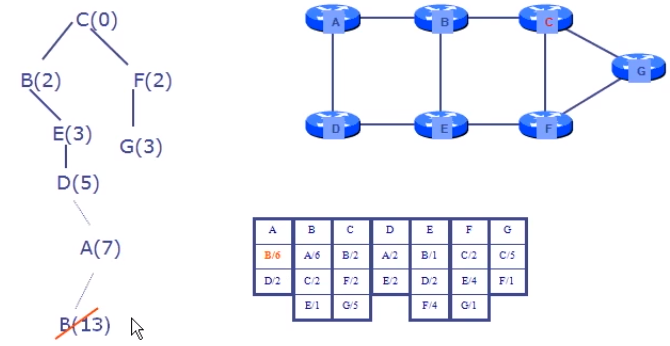
\includegraphics[width=0.8\linewidth]{IN1/IN75.png}
%\caption{Escalas de tiempo de los métodos para el control de la congestión.}
%\end{figure}
%\subsection{Enrutamiento consiente de tráfico}
%El objetivo es desviar el tráfico de los puntos más activos hacia otros, esto esta en desuso debido a su oscilación
%\begin{center}
%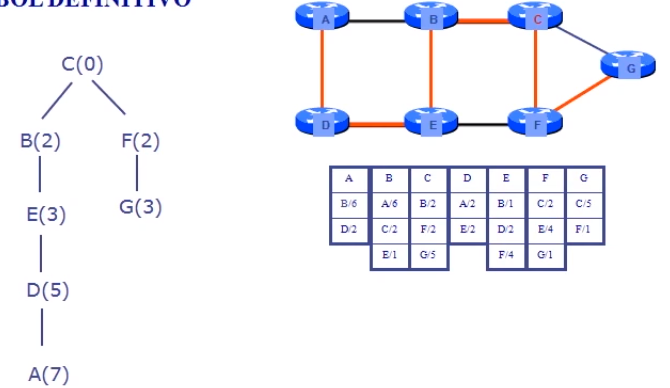
\includegraphics[width=0.8\linewidth]{IN1/IN76.png}
%\end{center}
%Sean dos sistemas autónomos como la image, los enlaces entre ambos sistemas son CF y EI, al congestionarse CF se enrutará los paquetes hacia EI para despejar CF. Pero luego de este proceso EI estará congestionado y verá EI como una ruta optima. El sistema de enrutamiento será \textbf{oscilatorio}.
%\subsection{Regulación de tráfico}
%\begin{figure}[H]
%\centering
%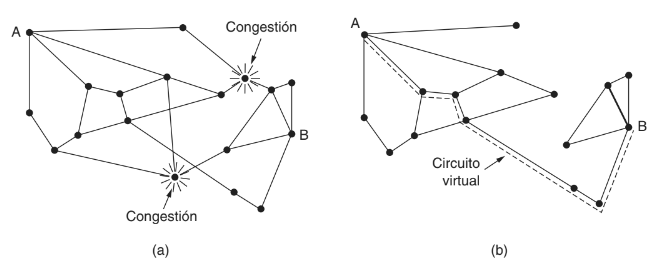
\includegraphics[width=\linewidth]{IN1/IN77.png}
%\caption{(a) Una red congestionada. (b) La parte de la red que no esta congestionada.}
%\label{fig:regulacion trafico}
%\end{figure}
%En la figura \ref{fig:regulacion trafico}.a se muestra la red con dos puntos de congestión, lo que haremos es eliminar esos puntos de congestión y calculando una nueva ruta virtual evitando los puntos de congestión. El problema puede ser que esta desviación tome un poco más de tiempo. Al existir una congestión, el router congestionado devuelve un trama al azar y envía un \textbf{paquete regulador} con un bit de encabezado al emisor para que no generé más paquetes y se reduzca el tráfico. Esto no es equitativo pues los emisor más rápidos tendrán más paquetes congestionados que lo emisores lentos.
%\subsubsection{ECN}
%ENC o notificación explicita de congestión, funciona similar al \textbf{paquete regulador}, en vez de crear un datagrama que vuelva al emisor, se configura dos bits para que cuando lleguen al receptor este se enteré en donde hubo una congestión y este mandará un mensaje al emisor directo para que tome las medidas.
%%%22:27l
%----------------------------------------------------------------------------------------
%Microprocesadores
%----------------------------------------------------------------------------------------

%----------------------------------------------------------------------------------------
%Mantenimiento
%----------------------------------------------------------------------------------------
\section{Distribución de Weibull}\index{Distribución de Weibull}
\begin{definition}[Función densidad probabilidad]
\begin{equation}
f(t,\alpha,\lambda)=\frac{\alpha}{\lambda^{\alpha}}t^{\alpha-1}e^{-\left(\frac{t}{\lambda}\right)^{\alpha}}, t>0
\label{eq:fdp weibull}
\end{equation}
\end{definition}
Si resolvemos la ecuación \ref{eq:fdp weibull} para t>0:
\begin{align*}
\frac{k}{\lambda^{\alpha}}\int_0^xt^{k-1}e^{-\left(\frac{t}{\lambda}\right)^{k}}&=u\\
\left(\frac{\beta}{\lambda^{k}}\right)\left(-\frac{\lambda^{k}}{k}\right)e^{-\left(\frac{t}{\lambda}\right)^{k}}\Big|_0^t&=u\\
1-e^{-\left(\frac{t}{\lambda}\right)^{k}}&=u
\intertext{Despejando se tiene:}
1-u&=e^{-\left(\frac{t}{\lambda}\right)^{k}}\\
1-u&=\frac{1}{e^{\left(\frac{t}{\lambda}\right)^{k}}}\\
e^{\left(\frac{t}{\lambda}\right)^{k}}&=\frac{1}{1-u}
\intertext{Tomando Log neperiano:}
Ln e^{\left(\frac{t}{\lambda}\right)^{k}}&=Ln\left(\frac{1}{1-u}\right)\\
\left(\frac{t}{\lambda}\right)^{k}&=Ln\left(\frac{1}{1-u}\right)\\
\frac{t^{k}}{\lambda^{k}}&=Ln\left(\frac{1}{1-u}\right)\rightarrow t^{k}=\lambda^{k}Ln\left(\frac{1}{1-u}\right)\\
t&=\lambda\left[Ln\left(\frac{1}{1-u}\right)\right]^{\frac{1}{k}}
\end{align*}
La distribución de Weibull es ampliamente usada en el estudio de tiempo de vida o tiempo de vida o tiempo para la falla de los componentes mecánicos. Los parámetros de la distribución de Weibull son: Forma ($k$ ó $\alpha$) y Escala ($\lambda$).\\
El número de ocurrencias de eventos por unidad de tiempo no permanece necesariamente constante, es decir, esta tasa de ocurrencia de eventos puede crecer o decrecer con el tiempo.
\begin{itemize}
\item R(t): Probabilidad de que el equipo no falle en un tiempo t. También se le llama \textbf{confiabilidad}.
\item $\lambda$: Parámetro de escala, vida característica del equipo.\footnote{No confundir con $\lambda$ de la función distribución.}
\item $k$: Parámetro de forma, relaciona el periodo de tiempo en el que se encuentra operando el equipo.
\item $\gamma$: También llamado parámetro de posición; define el punto de partida de la distribución.
\end{itemize}
\begin{table}[H]
\begin{center}
\begin{tabular}{|c|c|}
\hline
\rowcolor[HTML]{EFEFEF} 
Valor($k$)    & Carácteristicas                   \\ \hline
0<$k$<1       & Tasa de falla decreciente         \\ \hline
$k$=1         & Distribución exponencial          \\ \hline
1<$k$<2       & Tasa de falla creciente (concava) \\ \hline
$k$=2         & Distribución de Rayleigh          \\ \hline
$k$>2         & Tasa de falla creciente (convexa) \\ \hline
3$\leq k\leq$4 & Tasa de falla creciente           \\ \hline
\end{tabular}
\end{center}
\end{table}
\begin{figure}[H]
\centering
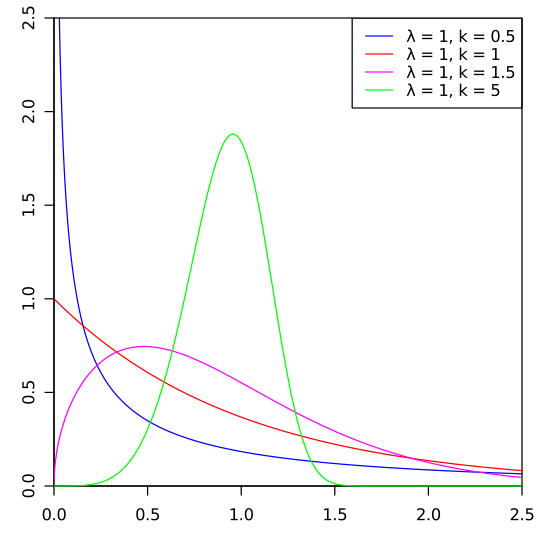
\includegraphics[width=.6\linewidth]{IM/IM37.png}
\caption{Distribución Weibull con diferentes valores de $k$ (k).}
\end{figure}
\subsection*{Propiedades de la distribución de Weibull}
De manera general
\begin{corollary}[Distribución]
\begin{equation}
f(t)=\frac{k}{\alpha^k}(t-\gamma)^{k-1}e^{\left(\frac{t-\gamma}{\alpha}\right)^{\beta}}
\end{equation}
\end{corollary}
\begin{corollary}[Infiabilidad]
\begin{equation}
F(t)=1-e^{-\left(\frac{t-\gamma}{\alpha}\right)^{\beta}}
\end{equation}
\end{corollary}
\begin{corollary}[Confiabilidad]
\begin{equation}
R(t)=e^{-\left(\frac{t-\gamma}{\alpha}\right)^{\beta}}
\end{equation}
\end{corollary}
\begin{corollary}[Tasa de fallas]
\begin{equation}
\lambda (t)=\frac{k}{\alpha^k}(t-\gamma)^{k-1}
\end{equation}
\end{corollary}
\begin{figure}[H]
\centering
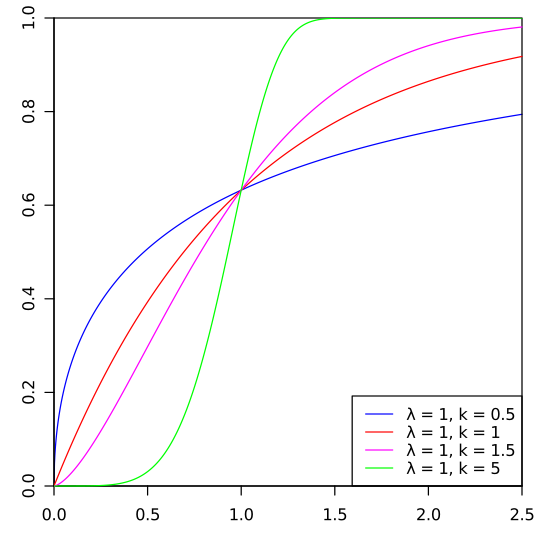
\includegraphics[width=0.8\linewidth]{IM/IM38.png}
\caption{CDF de una distribución de Weibull o Infiabilidad}
\end{figure}

\begin{table}[H]
\begin{center}
\begin{tabular}{|ccc|}
\hline
\rowcolor[HTML]{38FFF8} 
\multicolumn{3}{|c|}{\cellcolor[HTML]{38FFF8}Antena}                                                                                                                                                                                                                       \\ \hline
\rowcolor[HTML]{96FFFB} 
\multicolumn{1}{|c|}{\cellcolor[HTML]{96FFFB}Modo de fallo}                                                   & \multicolumn{1}{|c|}{\cellcolor[HTML]{96FFFB}Causa de fallo}                                                                            & Efecto de fallo   \\ \hline
\multicolumn{1}{|c|}{\begin{tabular}[c]{@{}l@{}}Desadaptación en el dipolo\\ con guía de onda\end{tabular}}   & \multicolumn{1}{l|}{\begin{tabular}[c]{@{}l@{}}Twist en el conector hacia el dipolo.\\ Conector con armado defectuoso.\end{tabular}}   & Corte del sistema \\ \hline
\multicolumn{1}{|l|}{Desorientación de antena}                                                                & \multicolumn{1}{l|}{\begin{tabular}[c]{@{}l@{}}Ajuste mecánico defectuoso en la abrazadera de\\ la antena hacia la torre\end{tabular}} & Corte del sistema \\ \hline
\multicolumn{1}{|l|}{\begin{tabular}[c]{@{}l@{}}Desadaptación del dipolo con\\ el espacio libre\end{tabular}} & \multicolumn{1}{l|}{\begin{tabular}[c]{@{}l@{}}Temperatura bajo el cero provoca granizo de hielo\\ en el dipolo\end{tabular}}          & Corte del sistema \\ \hline
\end{tabular}
\end{center}
\caption{Antenna}
\end{table}


\begin{table}[]
\begin{center}
\begin{tabular}{|ccc|}
\hline
\rowcolor[HTML]{38FFF8} 
\multicolumn{3}{|c|}{\cellcolor[HTML]{38FFF8}Guía de onda}                                                                                                                                                                                                                                                                                                                                                                                                                                         \\ \hline
\rowcolor[HTML]{96FFFB} 
\multicolumn{1}{|c|}{\cellcolor[HTML]{96FFFB}Modo de fallo}                                                        & \multicolumn{1}{c|}{\cellcolor[HTML]{96FFFB}Causa de fallo}                                                                                                                                                                            & Efecto de fallo                                                                                                                \\ \hline
\multicolumn{1}{|c|}{\begin{tabular}[c]{@{}c@{}}Desadaptación en el sistema Tx\\ guía de onda-dipolo\end{tabular}} & \multicolumn{1}{c|}{\begin{tabular}[c]{@{}c@{}}Sección elíptica asimétrica de la guía\\ ocasionado por el golpe en la superficie de la guía.\\ Exceso de radio de encorbatura en el tendido de la\\ guía hacia la torre.\end{tabular}} & \begin{tabular}[c]{@{}c@{}}Curva de retardo asimétrica\\ con ruptura.\\ Corte en el sistema por exceso \\ de ROE.\end{tabular} \\ \hline
\end{tabular}
\end{center}
\caption{Guía de onda}
\end{table}


%----------------------------------------------------------------------------------------
\end{document}
%----------------------------------------------------------------------------------------
